% !TeX program = xelatex
% !TEX TS-program = xelatex
% Compile with XeLaTeX or LuaLaTeX, twice for cross-references.
% Times New Roman where available; Times-compatible Liberation Serif otherwise.
% No platform-specific font paths or redistributed Windows fonts are required.
% Existing images are referenced without editing or copying source assets.
\documentclass[11pt,a4paper]{article}
\usepackage[margin=22mm]{geometry}
\usepackage{fontspec}
% Retain Times New Roman where available; use installed Liberation Serif otherwise.
\IfFontExistsTF{Times New Roman}{
  \setmainfont{Times New Roman}
  \setsansfont{Times New Roman}
  \setmonofont{Times New Roman}
}{
  \setmainfont{Liberation Serif}
  \setsansfont{Liberation Serif}
  \setmonofont{Liberation Serif}
}
\usepackage{amsmath,amssymb}
\usepackage{graphicx,float,caption,subcaption}
\usepackage{longtable,array,booktabs}
\usepackage{hyperref}
\hypersetup{hidelinks}
\usepackage{microtype}
\setlength{\emergencystretch}{3em}
\setlength{\parindent}{0pt}
\setlength{\parskip}{6pt}
\captionsetup{font=small,labelfont=bf}
% Paths are relative to the repository/Overleaf project root.
% Compile from that root; a missing image is an error, not a placeholder.
\newcommand{\projectimage}[2]{%
  \includegraphics[width=\linewidth,height=#2,keepaspectratio]{#1}%
}
\begin{document}
\section*{Supplementary Information}
{\large\bfseries Stage-Resolved Transcriptomic Analysis Reveals Distinct Molecular Programs Associated with Liver Fibrosis Severity\par}
\medskip
Authors: [AUTHOR NAMES AND AFFILIATIONS]
\medskip

\begingroup
\renewcommand{\thefigure}{S\arabic{figure}}
\renewcommand{\theHfigure}{supp.\arabic{figure}}
\setcounter{figure}{0}
\begin{figure}[H]\centering
\projectimage{task2_heatmap.pdf}{0.78\textheight}
\caption{\textbf{Fibrosis-stage expression-profile heatmap.} Row-standardised profiles of 3,845 fibrosis-associated genes across F0--F4, grouped into five clusters. The colour scale represents relative expression across stages; the profiles describe cross-sectional differences between patients.}\label{fig:S_heatmap}
\end{figure}
\clearpage
\begin{figure}[H]\centering
\projectimage{task2_choosing_k.pdf}{0.76\textheight}
\caption{\textbf{Cluster-number diagnostics.} Silhouette scores and adjusted Rand indices for $k=3$--8. Stability error bars show SD across 50 gene-subset or patient-bootstrap refits. The selected $k=5$ was the largest solution with mean gene-subset ARI $\geq0.95$; patient-bootstrap stability was assessed separately. Numerical values are reported in Supplementary Table~\ref{tab:S1}.}\label{fig:S_k}
\end{figure}
\clearpage
\begin{figure}[H]\centering
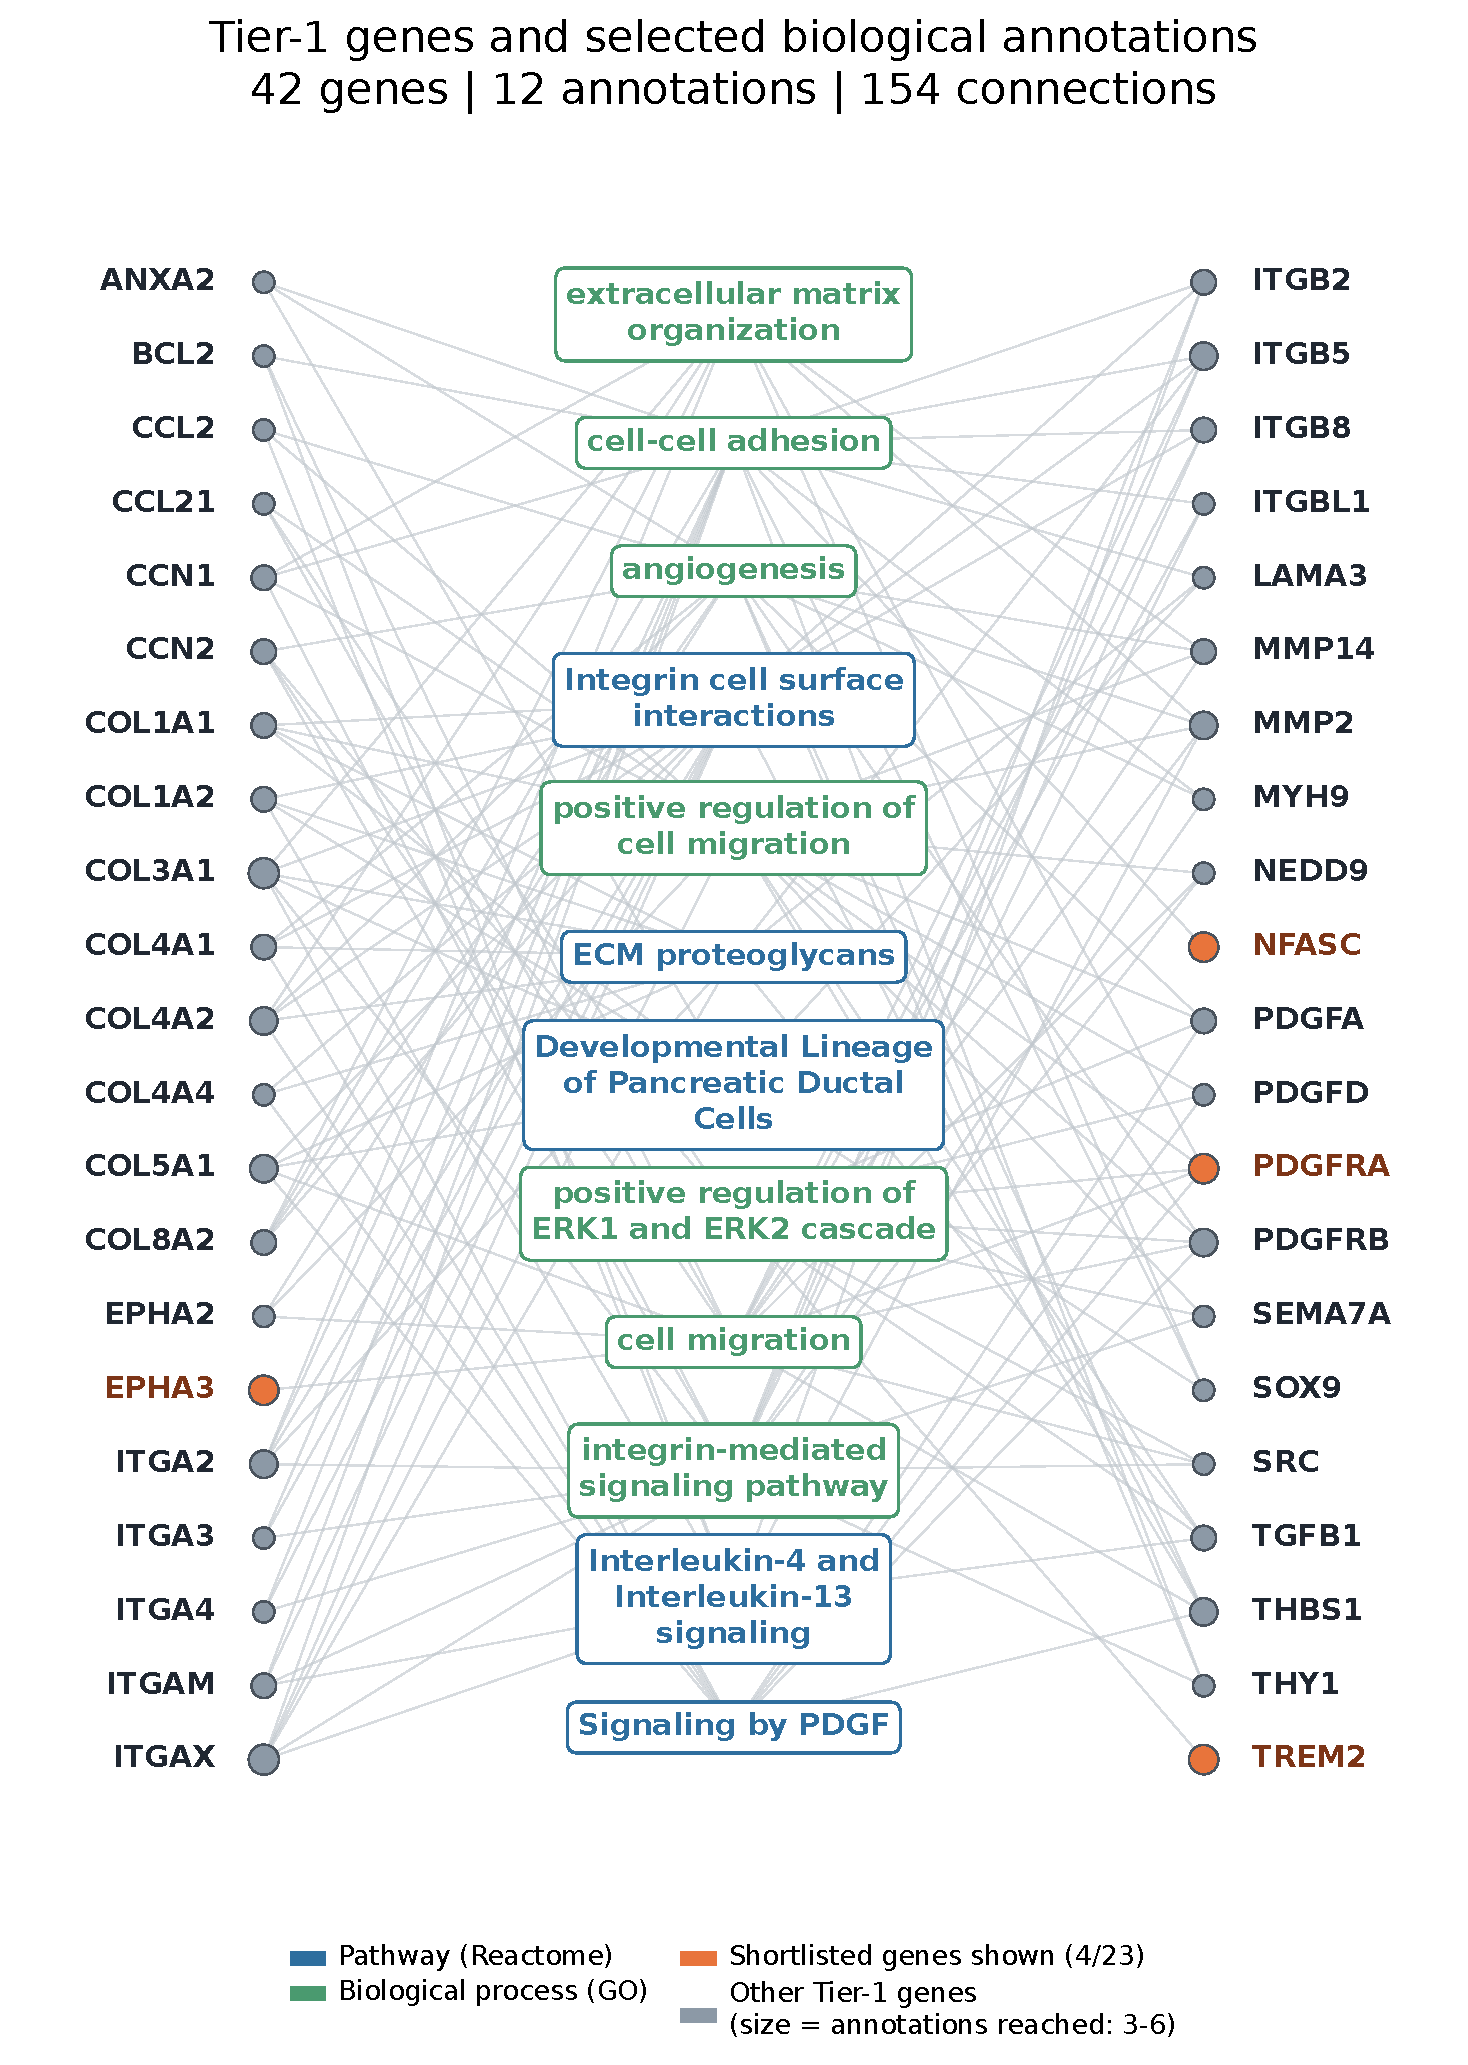
\includegraphics[width=\linewidth,height=0.80\textheight,keepaspectratio]{12_mechanistic_subgraph.pdf}
\caption{\textbf{Prioritised gene--annotation network.} Curated connections link 42 Tier 1 genes to twelve annotations through 154 relationships. Displayed genes reach at least three selected annotations, or are shortlisted genes reaching at least one. Connections represent annotation membership, not demonstrated physical or causal interactions.}\label{fig:5}
\end{figure}
\endgroup
\clearpage
\begingroup
\renewcommand{\thetable}{S\arabic{table}}
\renewcommand{\theHtable}{S\arabic{table}}
\setcounter{table}{0}
\begin{table}[H]\centering
\caption{Cluster-number diagnostics for all evaluated solutions}\label{tab:S1}
\fontsize{9}{11}\selectfont
\begin{tabular}{>{\raggedright\arraybackslash}p{0.045\textwidth}>{\raggedright\arraybackslash}p{0.13\textwidth}>{\raggedright\arraybackslash}p{0.245\textwidth}>{\raggedright\arraybackslash}p{0.245\textwidth}>{\raggedright\arraybackslash}p{0.13\textwidth}}
\toprule
\textbf{k} & \textbf{Silhouette} & \textbf{Gene-subset ARI (mean $\pm$ SD)} & \textbf{Patient-bootstrap ARI (mean $\pm$ SD)} & \textbf{Gene-subset mean ARI $\geq0.95$} \\
\midrule
3 & 0.5874 & 0.9811 $\pm$ 0.0183 & 0.7913 $\pm$ 0.0627 & Yes \\
4 & 0.4378 & 0.9708 $\pm$ 0.0174 & 0.6787 $\pm$ 0.0806 & Yes \\
5 & 0.3522 & 0.9835 $\pm$ 0.0107 & 0.5919 $\pm$ 0.0623 & Yes \\
6 & 0.3167 & 0.8164 $\pm$ 0.1717 & 0.5137 $\pm$ 0.0727 & No \\
7 & 0.2804 & 0.9343 $\pm$ 0.0452 & 0.4495 $\pm$ 0.0478 & No \\
8 & 0.2841 & 0.8676 $\pm$ 0.1104 & 0.4257 $\pm$ 0.0455 & No \\
\bottomrule
\end{tabular}
\par\vspace{6pt}
\begin{minipage}{0.94\textwidth}\small
Gene-subset diagnostics used 50 refits with 80\% of genes; patient-bootstrap diagnostics used a separate 50 refits resampling patients within studies. Values are reproduced from the cluster-number diagnostics, without reclustering. The selection rule chose the largest k with mean gene-subset ARI at least 0.95: k = 5. The highest silhouette score occurred at k = 3; patient-bootstrap ARI was not the selection criterion. Means and SDs are rounded to four decimal places for display; eligibility was assessed using the unrounded means.
\end{minipage}
\end{table}
\endgroup

\clearpage
\begingroup
\renewcommand{\thetable}{S\arabic{table}}
\renewcommand{\theHtable}{S\arabic{table}}
\setcounter{table}{1}
\fontsize{9}{11}\selectfont
\setlength{\tabcolsep}{4pt}
\renewcommand{\arraystretch}{1.15}
\begin{longtable}{>{\raggedright\arraybackslash}p{0.13\textwidth}>{\raggedright\arraybackslash}p{0.23\textwidth}>{\raggedright\arraybackslash}p{0.39\textwidth}>{\centering\arraybackslash}p{0.075\textwidth}>{\centering\arraybackslash}p{0.075\textwidth}}
\caption{Dataset-specific preprocessing and final analysis eligibility}\label{tab:S2}\\
\toprule
\textbf{Dataset} & \textbf{Expression processing} & \textbf{Sample handling and eligibility} & \textbf{Fibrosis\newline n} & \textbf{Disease\newline group n} \\
\midrule\endfirsthead
\multicolumn{5}{l}{\textbf{Table S2 continued}}\\
\toprule
\textbf{Dataset} & \textbf{Expression processing} & \textbf{Sample handling and eligibility} & \textbf{Fibrosis\newline n} & \textbf{Disease\newline group n} \\
\midrule\endhead
\bottomrule\endfoot
GSE126848 & Raw counts; CPM rescaling; $\log_2(\mathrm{CPM}+1)$ & Twelve obese-only samples excluded from ordered disease-group analysis. Fibrosis stages unavailable. & 0 & 45 \\
GSE130970 & TPM; $\log_2(\mathrm{TPM}+1)$ & Five ambiguous disease classifications marked unclassified; fibrosis stages retained. Remaining disease labels are histology-derived proxies. & 78 & 73 \\
GSE135251 & Deposited counts; CPM rescaling; $\log_2(\mathrm{CPM}+1)$ & Fibrosis annotations retained. Broad NAFLD labels excluded from ordered disease-group analysis, leaving only controls and no variation on that axis. & 216 & 0 \\
GSE162694 & Raw counts; CPM rescaling; $\log_2(\mathrm{CPM}+1)$ & Fibrosis annotations retained. Broad NAFLD labels excluded from ordered disease-group analysis, leaving only controls and no variation on that axis. & 143 & 0 \\
GSE167523 & Raw counts; CPM rescaling; $\log_2(\mathrm{CPM}+1)$ & All 98 NAFL/NASH-labelled observations eligible. Fibrosis stages unavailable. & 0 & 98 \\
GSE193066 & Deposited RLE-normalised counts; $\log_2(\mathrm{count}+1)$; no additional CPM rescaling & 164 biopsies resolved to 106 patient observations: 28 same-stage pairs averaged; 30 different-stage pairs represented by the first biopsy. No usable disease-group labels. & 106 & 0 \\
GSE240729 & Raw counts; CPM rescaling; $\log_2(\mathrm{CPM}+1)$ & All fibrosis-staged observations retained. No usable disease-group labels. & 67 & 0 \\
GSE269412 & Raw counts; CPM rescaling; $\log_2(\mathrm{CPM}+1)$ & Included in the expression resource; required clinical annotations unavailable for either association analysis. & 0 & 0 \\
\midrule
\textbf{Total} & --- & Final analytical observations within studies & \textbf{610} & \textbf{216} \\
\end{longtable}
\small
Counts refer to patient-level analytical observations within each study. Participant independence across accessions was not established. The two analysis populations overlap and must not be added together. Zero indicates no contribution to the specified association analysis, rather than exclusion from the expression resource. Input sample counts and source filenames are listed in Table~3.

For all datasets, duplicate raw gene identifiers were resolved by retaining the first occurrence. Gene identifiers were harmonised to Ensembl identifiers, and measurements from distinct identifiers mapping to the same sample--gene pair were summed before transformation. CPM library totals were calculated before mapping and filtering. Transformed expression was standardised per gene within each study ($\mathrm{ddof}=1$), followed by patient-level biopsy selection or averaging. GSE193066 standardisation used all 164 source biopsies before repeat-biopsy resolution. Study eligibility required at least 25 patient observations and variation on the relevant clinical axis.
\endgroup

\clearpage
\begingroup
\renewcommand{\thetable}{S\arabic{table}}
\renewcommand{\theHtable}{S\arabic{table}}
\setcounter{table}{2}
\fontsize{9}{11}\selectfont
\setlength{\tabcolsep}{4pt}
\renewcommand{\arraystretch}{1.15}
\begin{longtable}{>{\raggedright\arraybackslash}p{0.08\textwidth}>{\raggedright\arraybackslash}p{0.25\textwidth}>{\raggedright\arraybackslash}p{0.57\textwidth}}
\caption{Gene-prioritisation component scores and decision rules}\label{tab:S3}\\
\toprule
\textbf{Score} & \textbf{Evidence} & \textbf{Assignment rule} \\
\midrule\endfirsthead
\multicolumn{3}{l}{\textbf{Table S3 continued}}\\
\toprule
\textbf{Score} & \textbf{Evidence} & \textbf{Assignment rule} \\
\midrule\endhead
\bottomrule\endfoot
$P_g$ & Fibrosis-association magnitude & \textbf{2}: $|\operatorname{median}\rho|\geq0.40$. \textbf{1}: $0.30\leq|\operatorname{median}\rho|<0.40$. \textbf{0}: otherwise. Applied to genes already passing fibrosis-association discovery criteria. \\
$T_g$ & F0--F4 endpoint separation & Let $\Delta_g=\overline{z}_{F4}-\overline{z}_{F0}$. First require direction agreement with the median fibrosis correlation: both values positive or both non-positive. If agreement holds, assign \textbf{2} for $|\Delta_g|\geq1$, \textbf{1} for $0.5\leq|\Delta_g|<1$, and \textbf{0} otherwise. Direction disagreement assigns \textbf{0}. A zero difference receives \textbf{0} by magnitude. Cluster direction does not override this rule. \\
$X_g$ & Largest adjacent-stage contrast and matched-refit reproducibility & Select the full-data comparison with the largest available $|\beta|$. Define A: $q<0.05$ and $|\beta|\geq0.20$ in that comparison. Define B: at least 50\% of matched draws have $|\beta|\geq0.20$ and the same sign as the selected full-data coefficient. Assign \textbf{2} if A and B hold, \textbf{1} if exactly one holds, and \textbf{0} if neither holds. Matched-draw significance does not contribute. \\
$F_g$ & Operational fibrosis-only membership & \textbf{1}: selected in the fibrosis analysis but not in the ordered disease-group analysis. \textbf{0}: otherwise. This selection status does not establish biological specificity. \\
$B_g$ & Functional-annotation support & Count annotation collections containing at least one significantly enriched term (BH $q<0.05$) whose overlapping-gene list contains the gene, using its own concordant direction group or its full expression cluster. \textbf{2}: at least two collections; \textbf{1}: one; \textbf{0}: none. Eligible collections: GO Biological Process, KEGG legacy, Reactome and Hallmark. Each counts once across both routes; confidence-core enrichment is excluded. \\
\end{longtable}
\small
\textbf{Precision and thresholds.} Scoring uses exported median correlations and stage means recorded to three decimal places; the endpoint difference is also rounded to three decimals before comparison. Lower score thresholds are inclusive; statistical significance requires $q<0.05$.

\textbf{Contrast selection and missing evidence.} Exact ties in $|\beta|$ retain the first comparison in the order F0--F1, F1--F2, F2--F3, F3--F4. A missing full-data q-value does not satisfy condition A. Missing matched evidence for the selected contrast, or absence of a selected contrast, stops scoring rather than automatically assigning zero. All 3,845 fibrosis-associated genes had finite full-data coefficients and q-values for all four contrasts and matched evidence for the selected contrast.

\textbf{Annotation eligibility.} All significant terms are eligible, including terms not displayed in figures. Discordant shared genes have no concordant direction-group route but can receive support through their full expression cluster. Multiple terms within one collection do not increase its contribution.

\textbf{Total score and shortlist.} $S_g=P_g+T_g+X_g+F_g+B_g$ has a maximum of nine. Tier 1: $S_g\geq7$; Tier 2: $5\leq S_g<7$; Tier 3: $S_g<5$. Up to five Tier 1 genes per cluster are selected by descending total score, then descending absolute median fibrosis correlation. Clusters with fewer than five qualifying genes contribute fewer candidates. The components share evidence and do not constitute independent validation.
\endgroup

\clearpage
\begingroup
\renewcommand{\thetable}{S\arabic{table}}
\renewcommand{\theHtable}{S\arabic{table}}
\setcounter{table}{3}
\fontsize{9}{11}\selectfont
\setlength{\tabcolsep}{5pt}
\renewcommand{\arraystretch}{1.12}
\begin{longtable}{>{\raggedright\arraybackslash}p{0.65\textwidth}>{\raggedright\arraybackslash}p{0.25\textwidth}}
\caption{Final integrated graph composition and drug-annotation coverage}\label{tab:S4}\\
\toprule
\textbf{Measure} & \textbf{Count} \\
\midrule\endfirsthead
\multicolumn{2}{l}{\textbf{Table S4 continued}}\\
\toprule
\textbf{Measure} & \textbf{Count} \\
\midrule\endhead
\bottomrule\endfoot
Total nodes & 126,763 \\
Total relationships & 35,138,047 \\
Broad entity categories & 8 \\
Relationship types & 14 \\
Drug nodes & 12,544 \\
OptimusKG-derived Drug subset & 12,025 \\
Drug nodes from ChEMBL/DGIdb/GtoPdb/Open Targets integration & 519 \\
ACTS\_ON relationships (all sources) & 25,890 \\
OptimusKG-derived drug--gene records & 20,674 \\
Drug--gene records from ChEMBL/DGIdb/GtoPdb/Open Targets integration & 5,216 \\
Common source-list field & 25,890 \\
Common action-list field & 25,430 \\
Links from the four-database integration involving the 519 drugs & 846 \\
Links from the four-database integration involving OptimusKG drugs & 4,370 (2,104 drugs) \\
Expression relationships & 32,471,042 \\
Fibrosis / disease-group progression links & 3,845 / 4,199 \\
Displayed gene--annotation subgraph & 42 genes; 12 annotations; 154 links \\
\midrule
\multicolumn{2}{l}{\textbf{Populated fields among all 12,544 Drug nodes}}\\
SMILES & 9,036 \\
Molecule type & 12,051 \\
Maximum clinical phase & 10,293 \\
Approval flag & 9,902 \\
Withdrawal flag & 11,623 \\
Recovered name & 10,878 \\
\midrule
\multicolumn{2}{l}{\textbf{Populated fields on the 20,674 OptimusKG-derived drug--gene records}}\\
Direct-source, assertion, conflict and evidence-level fields & 20,674 each \\
Reference URLs & 2,893 \\
Mechanism text & 2,898 \\
\end{longtable}
\small
Counts were verified by direct queries of the integrated graph on 28 October 2026, including 12,544 Drug nodes and 25,890 \texttt{ACTS\_ON} relationships. Progression-link endpoints and reported properties were verified against the analysis exports for all 8,044 links; the displayed subgraph was verified by gene identifier, annotation identifier and relationship type. These checks establish consistency with the reported analyses rather than independent biological validation.

\textbf{Drug-source provenance.} Drug--gene evidence records GtoPdb 2026.3.1; DGIdb 5, interactions downloaded in October 2026; ChEMBL REST API, October 2026; and Open Targets Platform 26.09. These identifiers are reproduced from graph properties. The metadata-recovery implementation distinguishes OptimusKG recovery from ChEMBL gap filling.

\textbf{Coverage interpretation.} A populated approval or withdrawal flag may be true or false. A phase field does not establish current approval, availability or efficacy for liver disease. All drug entities use the Drug label; source properties distinguish their provenance. Missing metadata remain missing; property coverage uses the stated denominator. Drug annotations were not inputs to the transcriptomic association, clustering or P/T/X/F/B prioritisation procedures.
\endgroup

\subsection*{Supplementary Methods: implementation checks and reference-file inventory}
\paragraph{Ambiguous disease classifications.} The five GSE130970 samples assigned unclassified disease-group status in the primary analysis were GSM3758028, GSM3758038, GSM3758039, GSM3758073 and GSM3758074. Their original histological fields and fibrosis stages were retained.

\paragraph{Relationship schema.} The integrated graph used 14 relationship types: \texttt{EXPRESSES}, \texttt{IN\_DATASET}, \texttt{ASSOCIATED\_WITH}, \texttt{INTERACTS\_WITH}, \texttt{INVOLVED\_IN}, \texttt{IN\_PATHWAY}, \texttt{ACTS\_ON}, \texttt{TREATS}, \texttt{CONTRAINDICATED\_IN}, \texttt{OFF\_LABEL\_FOR}, \texttt{HAS\_PHENOTYPE}, \texttt{PARENT\_OF}, \texttt{TRACKS\_FIBROSIS} and \texttt{TRACKS\_INFLAMMATION}.

For transition scoring, the comparison with the largest absolute available full-data coefficient was selected, with ties resolved in the order F0--F1, F1--F2, F2--F3, F3--F4. A missing full-data q-value did not satisfy the substantial-difference condition. Missing matched evidence for the selected comparison, or the absence of a selected comparison for a gene, stopped scoring through an assertion rather than being assigned zero. In the final analysis, all 3,845 fibrosis-associated genes had finite coefficients and q-values for all four comparisons and matched evidence for the selected comparison. The reconstructed P/T/X/F/B scores agreed with the analysis table for all 3,845 genes.

The reference files read by the analysis scripts were \nolinkurl{data/raw/hgnc_complete_set.txt} (file modification date 20 August 2026; most recent gene-record modification date within the file 18 August 2026) and the OptimusKG parquet files in \nolinkurl{data/optimuskg} (file modification date 1 September 2026). SHA-256 checksums for all files are provided in the source manifest, \nolinkurl{source_checksums.txt}. File dates and checksums identify these retained files and do not establish official release dates.


\end{document}
